\documentclass{article}
\usepackage[utf8]{inputenc}
\usepackage[spanish]{babel}
\usepackage{listings}
\usepackage{graphicx}
\graphicspath{ {images/} }
\usepackage{cite}

\begin{document}

\begin{titlepage}
    \begin{center}
        \vspace*{1cm}
            
        \Huge
        \textbf{Taller de memoria}
            
        \vspace{0.5cm}
        \LARGE
            Informatica II
            
            
            Hecho por:
            
        \vspace{1.5cm}
            
        \textbf{Jean Carlos Perez Bustamante}
            
        \vfill
            
        \vspace{0.8cm}
            
        \Large
        Despartamento de Ingeniería Electrónica y Telecomunicaciones\\
        Universidad de Antioquia\\
        Medellín\\
        Septiembre de 2020
            
    \end{center}
\end{titlepage}



\section{Defina que es la memoria de computador}
la memoria es el dispositivo que retiene, memoriza o almacena datos informáticos durante algún periodo de tiempo.

\section{ Mencione los tipos de memoria que conoce y haga una pequeña descripción de cada tipo.}

\begin{itemize}
    \item Memoria RAM
    
    Conocida también como Random Access Memory (Memoria de Acceso Aleatorio), la memoria RAM es la memoria de almacenamiento temporal que guarda los programas y los datos que están siendo procesados, lo cual realiza solamente durante el procesamiento.

\begin{figure}[h]
    \centering
    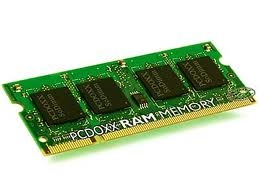
\includegraphics[width=0.5\textwidth]{ram.jpg}
    \caption{RAM}
    \label{fig:ram}
\end{figure}
    \item Memoria Cache
    El proceso que realiza la memoria caché es guardar las ubicaciones en el disco que ocupan los programas que han sido ejecutados, para que cuando vuelvan a ser iniciados el acceso a la aplicación logre ser más rápido.

    Existen tres tipos de caché diferentes:

    – El caché L1 que se encuentra en el interior del procesador y funciona a la misma velocidad que éste, y en el cual se guardan instrucciones y datos.

    – El caché L2 que suelen ser de dos tipos: interno y externo. El primero se encuentra dentro de la motherboard, mientras que el segundo se halla en el procesador pero de manera externa, lo que lo hace más lento que el caché L1.

    – El caché L3 que sólo vienen incorporado a algunos de los microprocesadores más avanzados, lo que resulta en una mayor velocidad de procesos.
    
\newpage
    
        \begin{figure}[h]
            \centering
            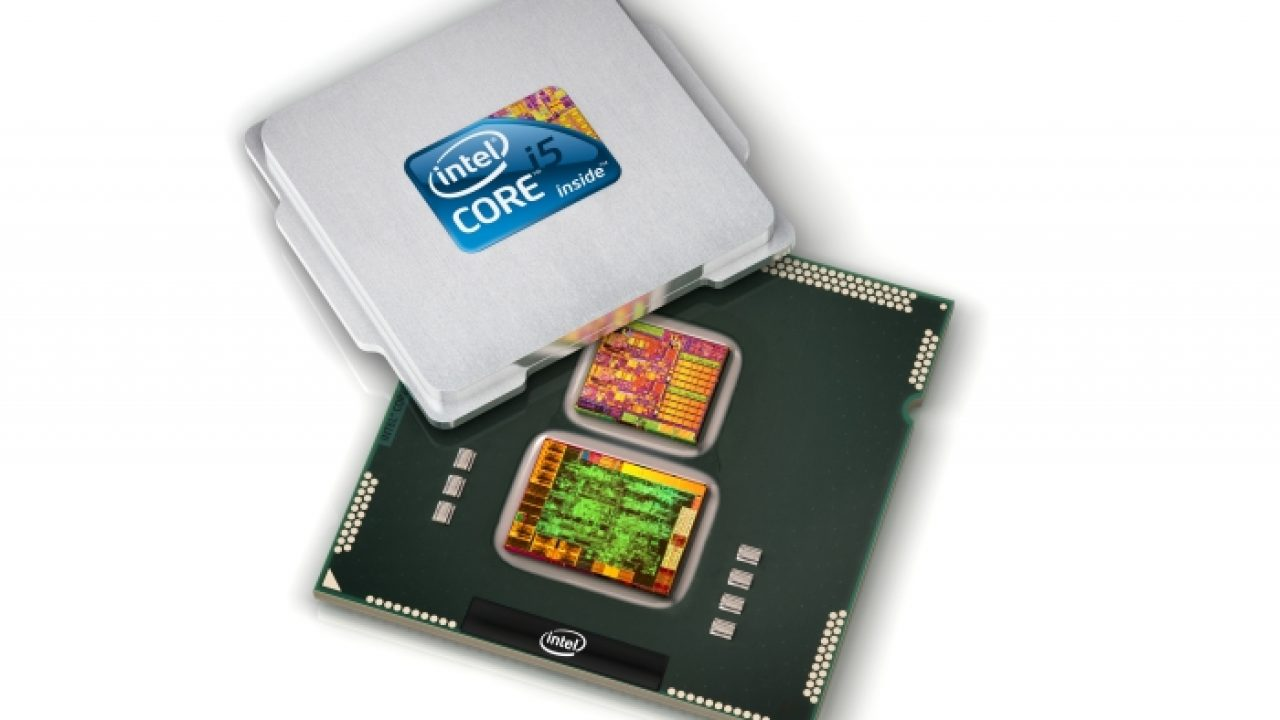
\includegraphics[width=0.5\textwidth]{cache.jpg}
            \caption{Memoria Cache}
            \label{fig:cache}
        \end{figure}
    
    \item Memoria ROM
    
    Read Only Memory, que como su nombre lo indica se trata de una memoria sólo de lectura, ya que la mayoría de estas memorias no pueden ser modificadas debido a que no permiten su escritura.
     La memoria ROM viene incorporada a la motherboard y es utilizada por la PC para dar inicio a la BIOS, lo cual es básicamente un programa que posee las instrucciones adecuadas para guiar a la computadora durante el arranque.

\begin{figure}[h]
    \centering
    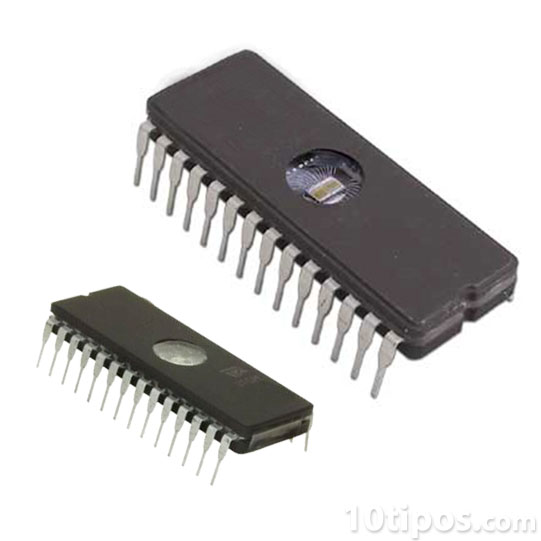
\includegraphics[width=0.5\textwidth]{rom.jpg}
    \caption{Memoria ROM}
    \label{fig:rom}
\end{figure}
\newpage

    \item Disco Duro
    
    Lo primero que tendremos que hacer es definir que es un disco duro. Un disco duro es un dispositivo para el almacenamiento de datos de forma no volátil, es decir, para almacenar los datos digitales utiliza un sistema de grabación magnética. De esta forma es posible mantener la información grabada en un soporte de forma permanente
    
    El disco duro está formado por uno o varios platos rígidos introducidos en una caja hermética y unidos por eje común que gira a gran velocidad. Sobre cada uno de los patos, que normalmente tienen sus dos caras destinadas al almacenamiento, se sitúan sendos cabezales de lectura/escritura.
    
    \begin{figure}[h]
        \centering
        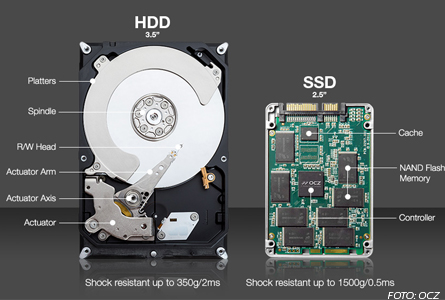
\includegraphics[width=0.5\textwidth]{disco.jpg}
        \caption{Hard Disk}
        \label{fig:disk}
    \end{figure}
    
    
    \end{itemize}
    
\newpage

\section{Describa la manera como se gestiona la memoria en un computador.}

Una memoria principal se compone de un conjunto de celdas básicas dotadas de una
determinada organización. Cada celda soporta un bit de información. Los bits se agrupan en unidades
direccionables denominadas palabras. La longitud de palabra la determina el número de bits que la
componen y constituye la resolución de la memoria (mínima cantidad de información direccionable).
La longitud de palabra suele oscilar desde 8 bits (byte) hasta 64 bits. 

\section{¿Qué hace que una memoria sea más rápida que otra? ¿Por qué esto es importante?}

Lo que hace que una memoria sea mas rapida que otra son las RPM Mientras mayor es el número de RPM, más rápido será el giro del disco y permitirá una lectura más rápida de dichos datos.esto hace que el proceso de latencia de una memoria sea mucho mas rapido, eso para el disco duro, en el caso de los otros tipos de memoria es similar entre mas rapido se d ela lectura de los bits, esta sera mas eficaz.

Es importante porque en la informatica se necesitan manejar muchos tipos de datos, en programas grandes seria una catastrofe que la memoria tarde en el proceso de compilacion, asi que se necesita el mejor rendimiento posible de la maquina para que todo salga bien, junto con el algoritmo hecho por la persona, se busca la mejor eficacia posible para los programas.


\section*{Referencias cruzadas}

En la imagen \ref{fig:ram} vemos una foto de la memoria RAM.

En la imagen \ref{fig:cache} vemos la foto de la memoria CACHE.

En la imagen \ref{fig:rom} vemos un dispositivo que es la memoria        ROM que se incrusta en una placa.

En la ultima imagen la cual es la \ref{fig:disk} vemos la imagen de el disco duro o tambien llamado Hard Disk, enumerando sus distintas partes que la componen.

\bibliographystyle{IEEEtran}
\bibliography{references}

http://www.fdi.ucm.es/profesor/jjruz/WEB2/Temas/EC5.pdf

https://www.tecnologia-informatica.com/tipos-memorias-computadora/

https://es.slideshare.net/MaryJoseSg/memoria-de-una-computadora




\end{document}
